\documentclass[
  a4paper,
  11pt,
]{memoir}

%%~~~~~~~~~~~~~~~~~~~~~~~~~~~~~~~~~~~~~~~~~~~~~~~~~~~~~~~~~~~~
%% Layout

%% For temporary redefining the geometry of titlepage, bibliography, and
%% backcover.  Have to include here, otherwise it resets the Memoir layout.
\usepackage{geometry}

%% Stock size is same as page (A4).
\settrims{0pt}{0pt}

%% Line length set in Charter for 65 chars is ~26.5pc.  We go as low as possible
%% to give room to the margins.  Height is as large as possible (we don't use
%% the footer).
\settypeblocksize{627pt}{26pc}{*}

%% 2cm spine is enough (we need space here!).
\setlrmargins{2cm}{*}{*}

%% Don't have an opinion on header yet.  Just not too near to body text.
%% \setheadfoot{\baselineskip}{0pt}
\setheaderspaces{*}{4pc}{*}

%% Yeah margin notes!
\setmarginnotes{2pc}{15pc}{1pc}

\checkandfixthelayout

%% Need this length for some full-width figures, and for headers
\newlength{\fullwidth}
\addtolength{\fullwidth}{\textwidth}
\addtolength{\fullwidth}{\marginparsep}
\addtolength{\fullwidth}{\marginparwidth}

%%~~~~~~~~~~~~~~~~~~~~~~~~~~~~~~~~~~~~~~~~~~~~~~~~~~~~~~~~~~~~
%% General typography

%% TTF fonts with XeLaTeX.
\usepackage{fontspec}

%% Charter is an amazing body font.
\setromanfont{Charter}

%% Fira Sans is nice for the titles.
\setsansfont[
  BoldFont=FiraSans-Medium,
  ItalicFont=FiraSans-BookItalic,
  BoldItalicFont=FiraSans-MediumItalic,
  Scale=MatchUppercase
]{Fira Sans Book}

%% A monospace font that handles utf8 chars.  And is not too wide.
%% Scaled to match the body font.
\setmonofont[Scale=MatchUppercase]{Fira Mono}

%% French typographical conventions and translated names for "Chapitre", "Table
%% des matières", etc.
\usepackage[main=french, english]{babel}

%% Move characters around and minimize hyphenation.  Good for diversity.  Not as
%% powerful with XeLaTeX, as font information may be missing.
\usepackage{microtype}

%% A touch of color
\usepackage{xcolor}
\definecolor{rubric}{rgb}{0.65,0.12,0.09}
\definecolor{azure}{rgb}{0.06,0.3,0.5}

%% Diagram colors
\definecolor{c0}{HTML}{556270}
\definecolor{c1}{HTML}{4ECDC4}
\definecolor{c2}{HTML}{FF6B6B}
\definecolor{c3}{HTML}{C7F464}

%%~~~~~~~~~~~~~~~~~~~~~~~~~~~~~~~~~~~~~~~~~~~~~~~~~~~~~~~~~~~~
%% Covers

%% Background image for first cover:
%% Paysage d'automne et d'hiver, Sesshū (end of 15th century)
\usepackage{eso-pic}
\newcommand\BackgroundPic{%
\put(0,0){%
\parbox[b][\paperheight]{\paperwidth}{%
\vfill
\centering
{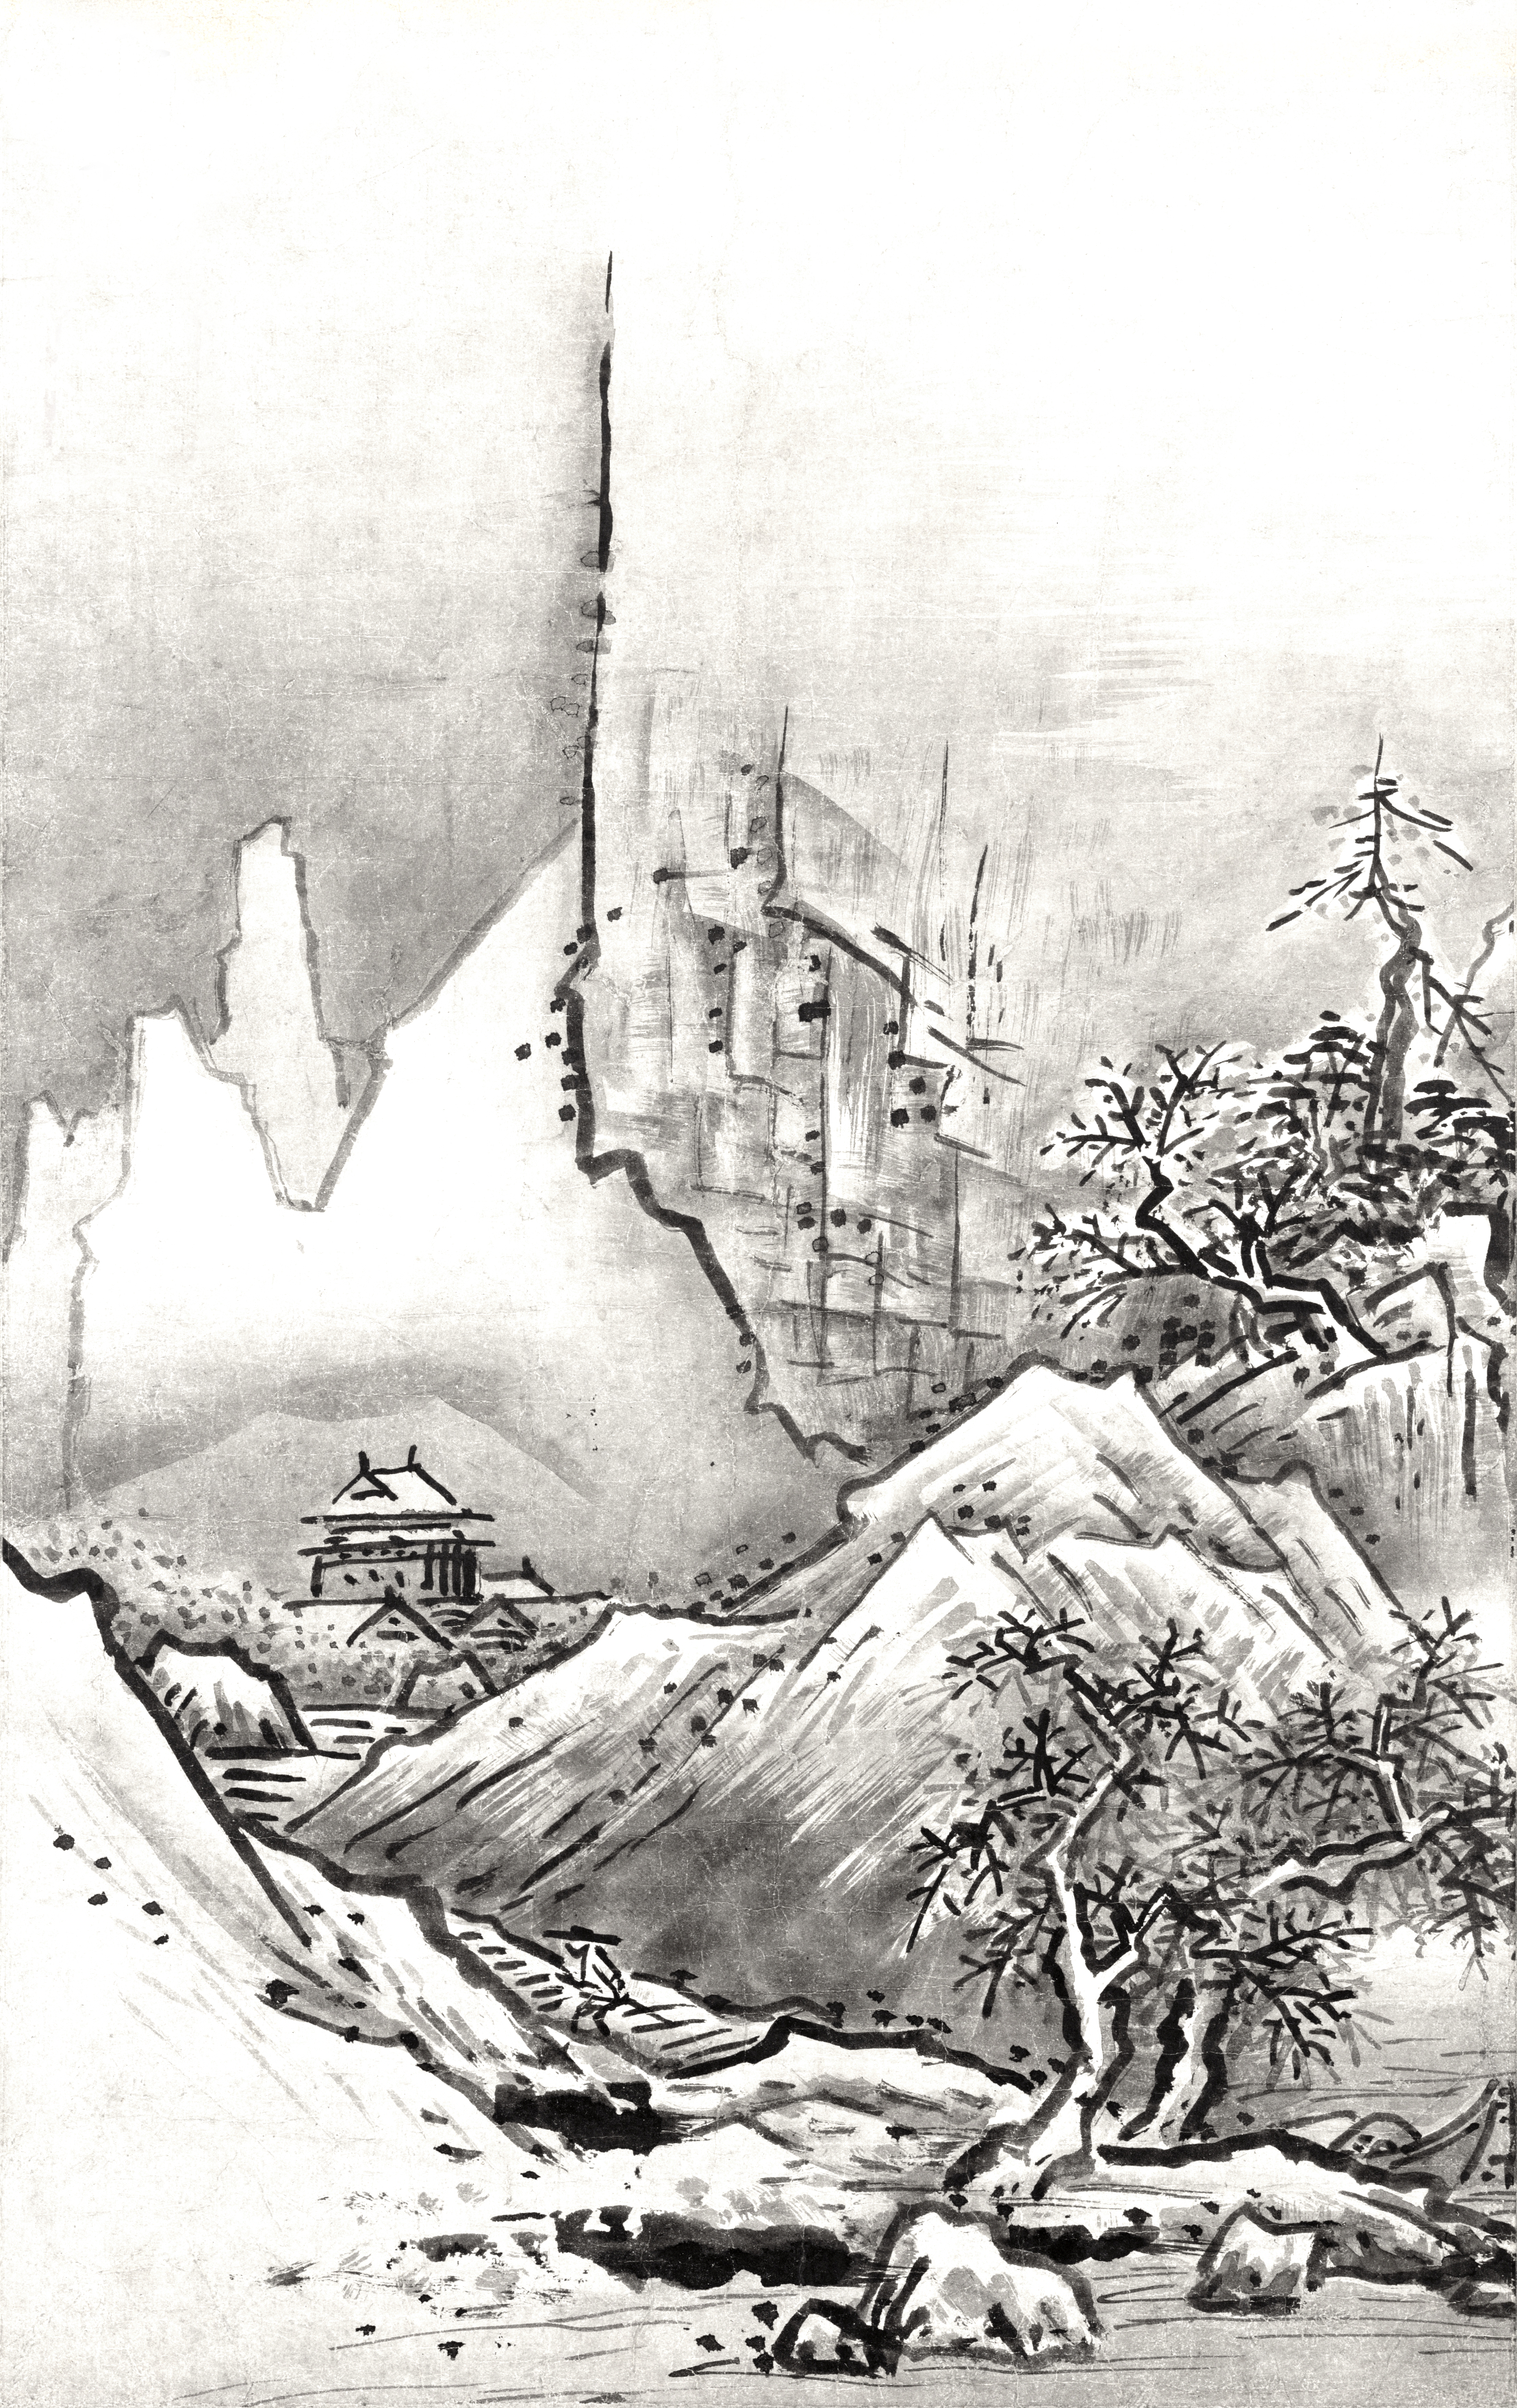
\includegraphics[width=\paperwidth,height=\paperheight,%
]{img/sesshu_sepia.jpg}}%
\vfill
}}}

%%~~~~~~~~~~~~~~~~~~~~~~~~~~~~~~~~~~~~~~~~~~~~~~~~~~~~~~~~~~~~
%% Page words (words instead of page numbers)

%% First read the leftover-words file that contains all the words.  The plan is
%% to map the page number N to the word at line N.  Thanks to:
%% https://tex.stackexchange.com/questions/17664/read-arbitrary-lines-from-file#17674
\makeatletter
\newread\myread
\newcount\linecnt
\openin\myread=leftover-words
\@whilesw\unless\ifeof\myread\fi{%
  \advance\linecnt by \@ne
  \readline\myread t\expandafter o\csname line-\number\linecnt\endcsname
}
\makeatother

%% Get the page word that corresponds to the given page number
%% For some reason (maybe readline?) there is an extra space at the end, hence
%% the final \hspace.
\newcommand{\pageword}[1]{\csname line-\number#1\endcsname\hspace{-3pt}}

%% Convenience to replace \thepage occurrences
\newcommand{\thepageword}{\pageword{\value{page}}}

%% Not settled yet, so might as well use a variable definition
\newcommand{\pagewordfont}{\sffamily\small}

%%~~~~~~~~~~~~~~~~~~~~~~~~~~~~~~~~~~~~~~~~~~~~~~~~~~~~~~~~~~~~
%% Table of contents

%% Insert page words in the ToC by redefining these functions provided by
%% memoir.
\let\oldchapterfpnum\cftchapterformatpnum
\renewcommand*{\cftchapterformatpnum}[1]{%
  \oldchapterfpnum{\pagewordfont\pageword{#1}}}

\let\oldsectionfpnum\cftsectionformatpnum
\renewcommand*{\cftsectionformatpnum}[1]{%
  \oldsectionfpnum{\pagewordfont\pageword{#1}}}

%% Sans-serif headings
\renewcommand*{\cftchapterfont}{\sffamily\bfseries}
\renewcommand*{\cftsectionfont}{\sffamily}

%%~~~~~~~~~~~~~~~~~~~~~~~~~~~~~~~~~~~~~~~~~~~~~~~~~~~~~~~~~~~~
%% Headings

%% Sans-serif headings
\headstyles{komalike}

%% In-your-face chapter style
\chapterstyle{pedersen}
\renewcommand{\chaptitlefont}{\Huge\sffamily\bfseries}
\renewcommand{\chapnumfont}{\sffamily\itshape}

%% Headers run into the margin thanks to the companion style of memoir.  I just
%% don't like the bold, so I redefine the font.
\makeevenhead{companion}%
             {\pagewordfont\thepageword}{}{%
               \sffamily\leftmark}
\makeoddhead{companion}%
            {\sffamily\rightmark}{}{%
              \pagewordfont\thepageword}

%% Don't use page words for front matter
%% FIXME: maybe for 3 pages of front matter we can just get rid of it
\makepagestyle{front}
\makeevenfoot{front}{}{\thepage}{}
\makeoddfoot{front}{}{\thepage}{}

%% Chapters use the plain pagestyle, and we want page words here as well
\makeoddfoot{plain}{}{\pagewordfont\thepageword}{}

%% For some reason, I can't get the ToC to use anything other than the plain
%% pagestyle.  Luckily, it's the only chapter that opens on an even page.
\makeevenfoot{plain}{}{\thepage}{}

%% Section headings run into the margin
\usepackage{calc}               % for widthof and minof

%% Wrapper around the checkoddpage functionality provided by memoir.
%% https://tex.stackexchange.com/questions/6143/if-then-else-for-odd-page-even-page
\strictpagecheck
\makeatletter
\newcommand*\ifthispageodd{%
  \checkoddpage
  \ifoddpage
    \expandafter\@firstoftwo
  \else
    \expandafter\@secondoftwo
  \fi
}
\makeatother

%% On odd page we just have to put the heading text into a fullwidth parbox to
%% let it run in the margin.  But on even pages, we want the /start/ of the
%% heading text to overrun into the left margin only if it is larger than
%% textwidth.
\newlength{\headingoffset}
\newcommand{\marginhead}[1]{%
  \ifthispageodd{\setlength{\headingoffset}{0pt}}
                {\setlength{\headingoffset}{%
                    \minof{0pt}{\textwidth-\widthof{#1}}}}
  \noindent\hspace{\headingoffset}
  \parbox{\fullwidth}{#1}}
%% This command overrides the font style, but here we just add the \marginhead
\setsecheadstyle{\sffamily\Large\bfseries\marginhead}

%%~~~~~~~~~~~~~~~~~~~~~~~~~~~~~~~~~~~~~~~~~~~~~~~~~~~~~~~~~~~~
%% Side notes (in the outer margin)

%% For hyphenation in ragged text, which gives more even side notes.
\usepackage{ragged2e}

%% Marginpar is touchy to align vertically.  Marginnote is easier.
\usepackage{marginnote}
\renewcommand*{\raggedleftmarginnote}{\RaggedLeft}
\renewcommand*{\raggedrightmarginnote}{\RaggedRight}
\renewcommand*{\marginfont}{\small}

%% To refer to the body text of an environment using \BODY.
\usepackage{environ}

%% Aside is for side commentary.  Like footnotes, but in the margin.
\NewEnviron{aside}[1][0pt]{\marginnote{\BODY}[#1]}

%% Side figures are an image and a caption, both in the margin.
\NewEnviron{side-figure}[1][0pt]{\marginnote{\BODY}[#1]}

%% Babel french puts it in small caps.  I don’t want that.
%% Additionally, override figurename for listings.
%% HACK: maybe using a new environment for the listings would be a better
%% solution.
%% \newcommand{\UnsetListingFigureName}{\renewcaptionname{french}{\figurename}{Figure}}
%% \UnsetListingFigureName
%% \newcommand{\SetListingFigureName}{\renewcaptionname{french}{\figurename}{Code}}

%%~~~~~~~~~~~~~~~~~~~~~~~~~~~~~~~~~~~~~~~~~~~~~~~~~~~~~~~~~~~~
%% Epigraphs

\NewEnviron{epig}[1][]{\epigraph{\BODY}{#1}}
\setlength{\epigraphwidth}{20pc}
\setlength{\epigraphrule}{0pt}

%%~~~~~~~~~~~~~~~~~~~~~~~~~~~~~~~~~~~~~~~~~~~~~~~~~~~~~~~~~~~~
%% Source code listings

%% Environment for source code snippets.
\usepackage{listings}
\lstset{
  basicstyle=\ttfamily\small,
  commentstyle=\ttfamily\color{rubric},
  keywordstyle=,
  columns=spaceflexible, keepspaces=true,
  breaklines=false, showstringspaces=false,
  escapeinside={//*}{\^^M},     % Escape to LaTeX between //* and line return
  numbersep=5pt,
  numberstyle=\scriptsize,
  %% aboveskip=-4pt,               % No space above and below, symmetric
  %% belowskip=0pt,
  %extendedchars=true, inputencoding=utf8,
}

%% Org export produces environment for ‘js’, so we must define that language for
%% listings.
\lstdefinelanguage{js}{
  language={Java},
  morekeywords={with,var,function},
  deletekeywords={double},
}

%% Accept the following’ as languages, no special treatment.  Otherwise listings
%% refuses to compile.
\lstdefinelanguage{diff}{}
\lstdefinelanguage{smalltalk}{}
\lstdefinelanguage{rust}{}
\lstdefinelanguage{elisp}{}
\lstdefinelanguage{asm}{}
\lstdefinelanguage{fortran}{}
\lstdefinelanguage{none}{}

%%~~~~~~~~~~~~~~~~~~~~~~~~~~~~~~~~~~~~~~~~~~~~~~~~~~~~~~~~~~~~
%% Bibliography

%% Quells a warning from biblatex with babel activated.  Not sure /what/ it does
%% though.
\usepackage{csquotes}

%% Generates the bibliography.  Handles UTF8-encoded bib files.
\usepackage[
  backend=biber,
  firstinits=false,
  sorting=nyt,                  % Sort by name, year, title
  backref=true,
  citestyle=alphabetic,
  bibstyle=alphabetic-pagewords, % Custom Biblatex style that handles pagewords
  maxbibnames=10
]{biblatex}
\addbibresource{refs.bib}

%% Smaller URLs in bibliography.  URLs in the body text are still in serif.
\renewcommand{\UrlFont}{\small\ttfamily}

%%~~~~~~~~~~~~~~~~~~~~~~~~~~~~~~~~~~~~~~~~~~~~~~~~~~~~~~~~~~~~
%% Others

%% Needed for the \text command in math-mode.
\usepackage{amsmath}

%% For including SVG (that are converted as PDF), and the JPEG illustrations.
\usepackage{graphicx}
%% This allows us to use width=\maxwidth{len} in \includegraphics to emulate the
%% CSS property max-width used by the HTML output.
%% Thanks: https://tex.stackexchange.com/questions/86350/includegraphics-maximum-width#86355
\makeatletter
\def\maxwidth#1{\ifdim\Gin@nat@width>#1 #1\else\Gin@nat@width\fi}
\makeatother

%% For color legend in diagrams
\newcommand{\colorrule}[1]{\textcolor{#1}{\rule{8pt}{4pt}}}

%% Hyperlinks for citations and external links.
\usepackage{hyperref}
\hypersetup{
  unicode,                      % Always a good idea?
  colorlinks=true,              % Color links rather than put boxes around them
  linkcolor=rubric,             % internal link
  citecolor=rubric,             % bibliography link
  urlcolor=azure,               % external link
  %% hidelinks=true,               % For printing only
}

%% Temporary handling of special blocks.
\newenvironment{full-figure}{}{}

%% Drop any FIXME.  The PDF is for reading!
\NewEnviron{fixme}{}
